\providecommand{\main}{..}
\documentclass[\main/main.tex]{subfiles}
\begin{document}

\chapter{Results}
\section{Reproducing the results}
Test were run on multiple datasets, all containing non-structured textual documents. All tests were run via the \href{https://github.com/LucaCappelletti94/zipf_classifier/blob/master/test.py}{test.py} file, available in the github repository, with the following parameters:
\begin{description}
	\item[Seed] The random uniform generator used to split files, run kmeans etc\ldots were initialized to \(1242\).
	\item[Training percentage] Of every dataset, \(70\%\) of the documents were used for training the classifier. The remaining \(30\%\) were used for testing. The split of the training and testing datasets was done selecting documents following an uniform random distribution initialized with the seed above.
	\item[Kmeans clusters \(k\)] For every test, \(10\) clusters were used.
	\item[Kmeans iterations] For every test \(100\) iterations were run before assuming convergence. Better results may be obtained with more iterations.
	\item[CURE representatives percentage] For every test \(10\%\) of the training points were used as representative points.
	\item[CURE distance percentage] For every test chosen representative points were moved \(20\%\) towards their respective centroids.
\end{description}

The complete dataset is available at the following url:

\url{https://mega.nz/#!XCI3iCiZ!EpBtedozqBivPcWYi8oAj6jx38LAJnUaNDfjvgzJi3I}.

The already trained classifiers are available at the following url:

\url{https://mega.nz/#!yLAR0CSI!4g6jNfTeTpoEbss3P4jmuJyvTvv0Wmtw1sZQydQS1Qs}.

\clearpage
\section{Authors}
The ``authors'' dataset contains \(315\) texts from 3 authors: D. H. Lawrence, Mark Twain and Oscar Wilde. Each author has \(105\) documents.
\subsection{Confusion matrix}
\begin{figure}
	\begin{subfigure}{0.40\textwidth}
		\includegraphics[width=\textwidth]{matrix/testing-datasets_authors.png}
		\caption{Confusion matrix for dataset ``authors''}
	\end{subfigure}
	\begin{subfigure}{0.40\textwidth}
		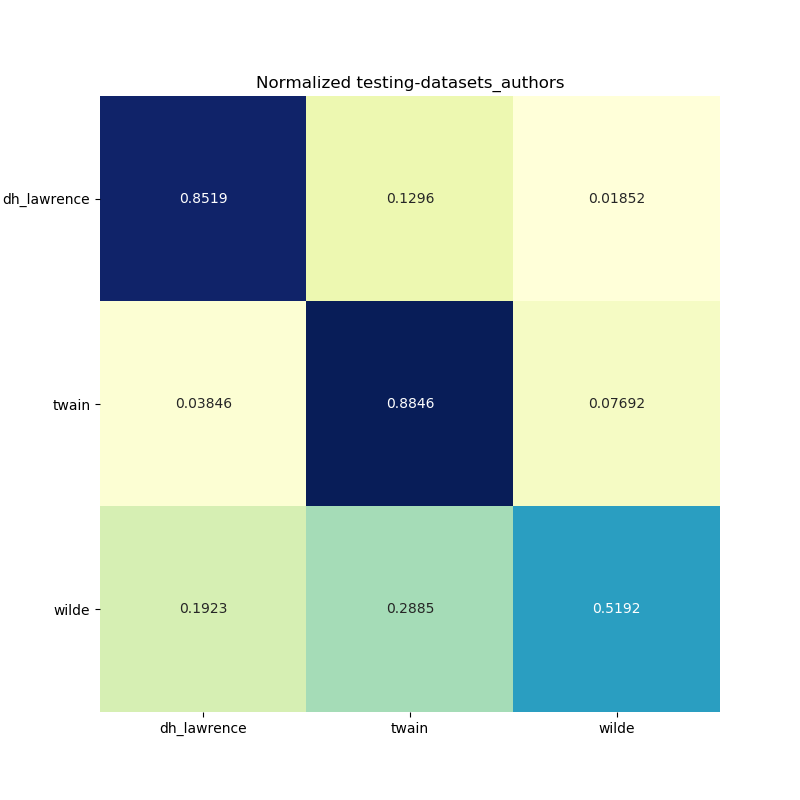
\includegraphics[width=\textwidth]{matrix/Normalized_testing-datasets_authors.png}
		\caption{Confusion matrix for dataset ``authors''}
	\end{subfigure}
	\caption{Ctrix for datascest ``authors''}
\end{figure}
\subsection{Truncated SVD reduction}
\begin{figure}
	\includegraphics[width=\textwidth]{svd/testing-datasets_authors.png}
	\caption{Dimensionality reduction using truncated SVD in dataset ``authors''}
\end{figure}

\clearpage
\section{Literary periods}
The ``literary periods'' dataset contains \(1060\) texts from 4 literary periods: Modernism, Realism, Romanticism and Naturalism. Each period has \(265\) documents.
\subsection{Confusion matrix}
\begin{figure}
	\begin{subfigure}{0.40\textwidth}
		\includegraphics[width=\textwidth]{matrix/testing-datasets_periods.png}
		\caption{Confusion matrix for dataset ``literary periods''}
	\end{subfigure}
	\begin{subfigure}{0.40\textwidth}
		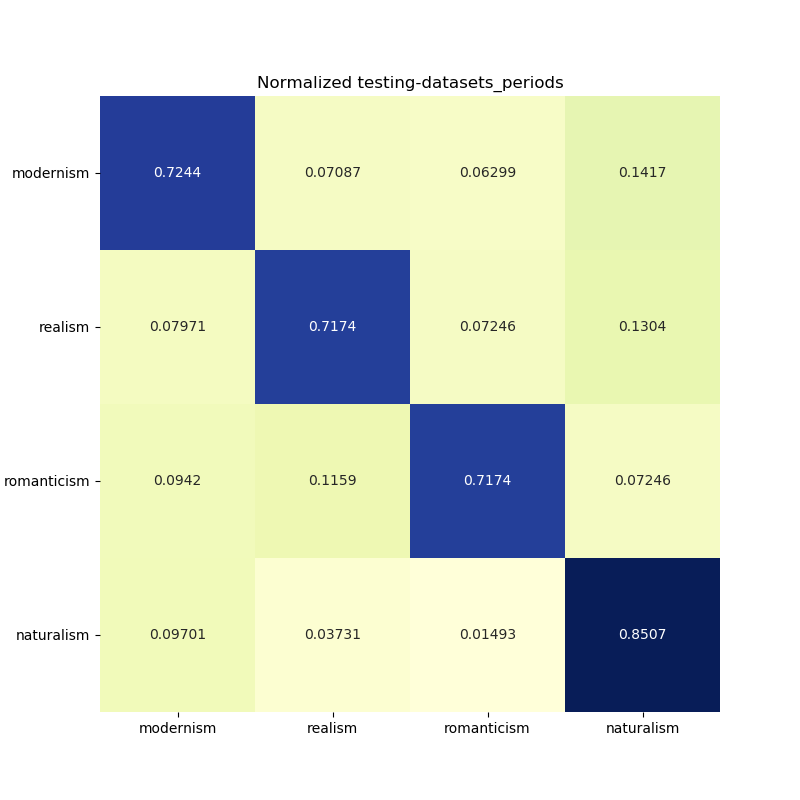
\includegraphics[width=\textwidth]{matrix/Normalized_testing-datasets_periods.png}
		\caption{Normalized confusion matrix for dataset ``literary periods''}
	\end{subfigure}
	\caption{Confusion matrices for dataset ``literary periods''}
\end{figure}
\subsection{Truncated SVD reduction}
\begin{figure}
	\includegraphics[width=\textwidth]{svd/testing-datasets_periods.png}
	\caption{Dimensionality reduction using truncated SVD in dataset ``literary periods''}
\end{figure}

\clearpage
\section{Recipes websites}
The ``recipes websites'' dataset contains \(12768\) texts from 4 italian websites dedicated to recipes: Misya, Salepepe, Zafferano and Lacucinaitaliana. Every website in the dataset has \(3192\) texts.
\subsection{Confusion matrix}
\begin{figure}
	\begin{subfigure}{0.40\textwidth}
		\includegraphics[width=\textwidth]{matrix/testing-datasets_recipes_websites.png}
		\caption{Confusion matrix for dataset ``recipes websites''}
	\end{subfigure}
	\begin{subfigure}{0.40\textwidth}
		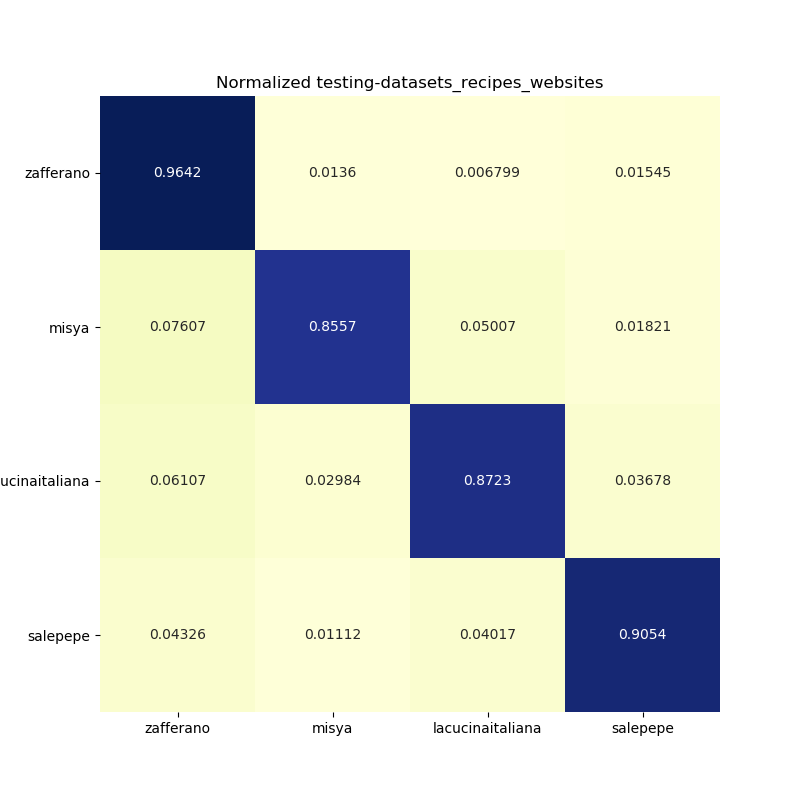
\includegraphics[width=\textwidth]{matrix/Normalized_testing-datasets_recipes_websites.png}
		\caption{Normalized confusion matrix for dataset ``recipes websites''}
	\end{subfigure}
	\caption{Confusion matrices for dataset ``recipes websites''}
\end{figure}
\subsection{Truncated SVD reduction}
\begin{figure}
	\includegraphics[width=\textwidth]{svd/testing-datasets_recipes_websites.png}
	\caption{Dimensionality reduction using truncated SVD in dataset ``recipes websites''}
\end{figure}

\clearpage
\section{Newspaper websites}
The ``newspaper websites'' dataset contains \(28000\) texts from 4 italian news websites: Repubblica.it, Moto.it, Scienze.it and Gazzetta.it. Every website in the dataset has \(7000\) texts.
\subsection{Confusion matrix}
\begin{figure}
	\begin{subfigure}{0.40\textwidth}
		\includegraphics[width=\textwidth]{matrix/testing-datasets_various_websites.png}
		\caption{Confusion matrix for dataset ``newspaper websites''}
	\end{subfigure}
	\begin{subfigure}{0.40\textwidth}
		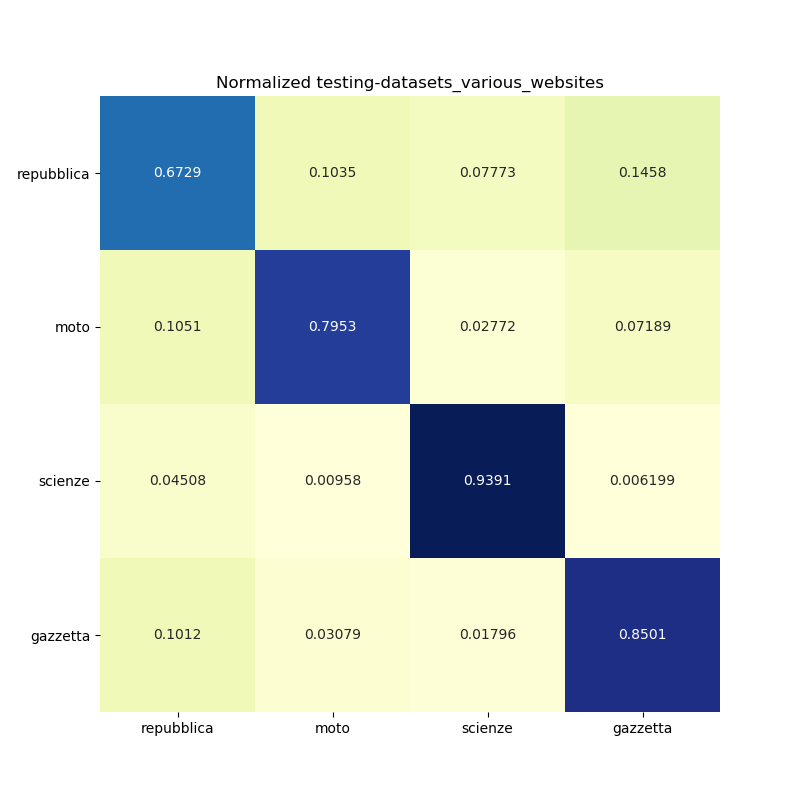
\includegraphics[width=\textwidth]{matrix/Normalized_testing-datasets_various_websites.png}
		\caption{Normalized confusion matrix for dataset ``newspaper websites''}
	\end{subfigure}
	\caption{Confusion matrices for dataset ``newspaper websites''}
\end{figure}
\subsection{Truncated SVD reduction}
\begin{figure}
	\includegraphics[width=\textwidth]{svd/testing-datasets_various_websites.png}
	\caption{Dimensionality reduction using truncated SVD in dataset ``newspaper websites''}
\end{figure}

\clearpage
\section{Recipes websites or non recipes websites}
This dataset contains \(36000\) texts, with two classes: recipes and non-recipes. Each class has \(18000\) texts.
\subsection{Confusion matrix}
\begin{figure}
	\begin{subfigure}{0.40\textwidth}
		\includegraphics[width=\textwidth]{matrix/testing-datasets_recipes.png}
		\caption{Confusion matrix for dataset ``recipes''}
	\end{subfigure}
	\begin{subfigure}{0.40\textwidth}
		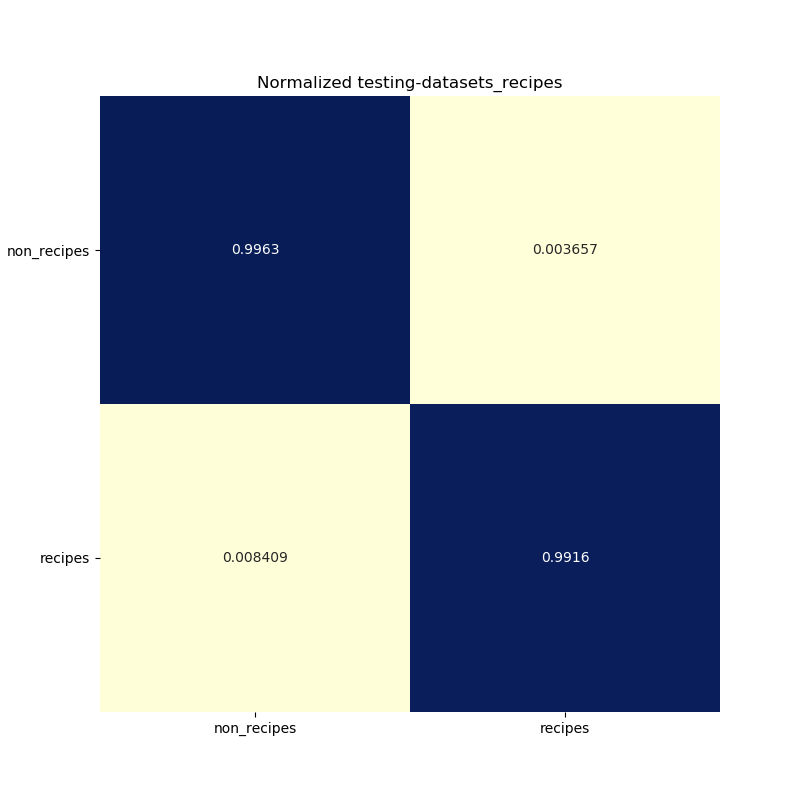
\includegraphics[width=\textwidth]{matrix/Normalized_testing-datasets_recipes.png}
		\caption{Normalized confusion matrix for dataset ``recipes''}
	\end{subfigure}
	\caption{Confusion matrices for dataset ``recipes''}
\end{figure}
\subsection{Truncated SVD reduction}
\begin{figure}
	\includegraphics[width=\textwidth]{svd/testing-datasets_recipes.png}
	\caption{Dimensionality reduction using truncated SVD in dataset ``recipes''}
\end{figure}

\end{document}